\clearpage
%%%%%%%%%%%%%%%%%%%%%%%%%%%%%%%%%%%%%%%%%%%%%%%%%%%%%%%%%%%%%%%%%%%%%%%%%%%%%%%%%
\begin{figure}[htbp]
    \section{Intune for Education}
    \label{sec:IntuneforEducation}

    \hspace{8pt} Intune for Education は、教育機関が自分たちのWindows 10 デバイスや iPad などを効率的に管理するためのクラウドサービスです。Inture for Education は教育機関がデバイスを管理しやすいようにカスタマイズされています。どのような規模の学校であってもWindows 10 デバイスの初期設定を簡単に行うことができ、継続的な管理ができるようになっています。

    \hspace{8pt} システム管理者は、アプリケーションを端末に展開したり、デバイスやユーザーごとに設定をカスタマイズすることができます。

    \hspace{8pt} Intune for Education の\textbf{「高速構成」}では、教育機関で最も利用される設定のみが表示され、推奨設定も提供されております。
\end{figure}
%%%%%%%%%%%%%%%%%%%%%%%%%%%%%%%%%%%%%%%%%%%%%%%%%%%%%%%%%%%%%%%%%%%%%%%%%%%%%%%%%

\begin{figure}[htbp]
    \subsection{Intune for Education で設定できること}
    \label{sec:IntuneforEducationでできること}

    Intune for Educationではアプリケーションの展開以外に以下のことを設定することができます。
\end{figure}

\begin{figure*}[htbp]
    \centering
    \vspace{-11cm}
    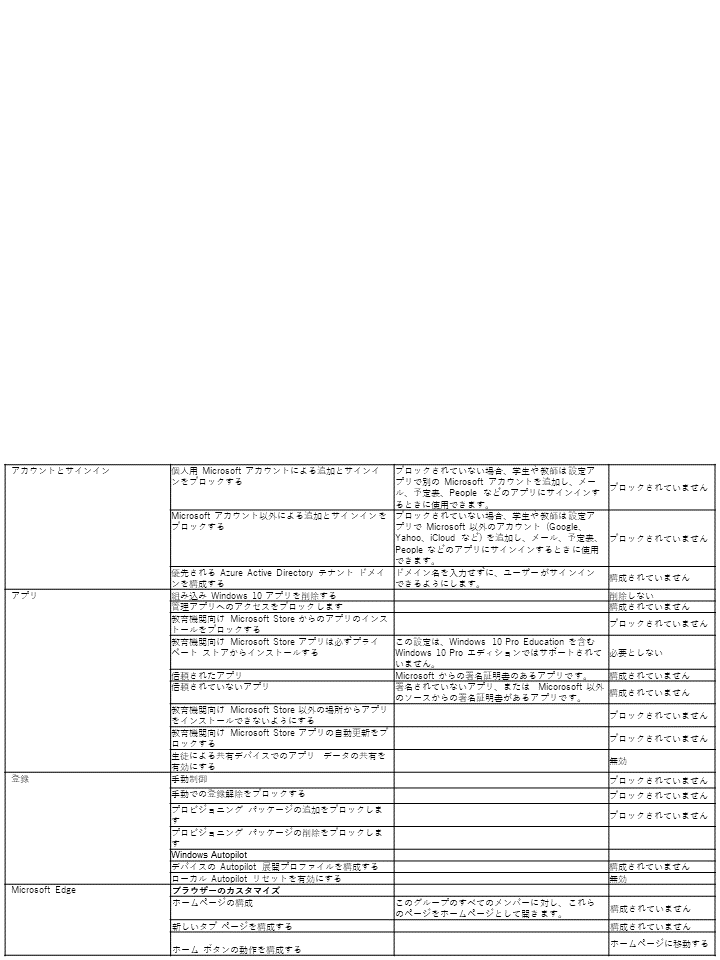
\includegraphics[width=17cm]{figures/IntuneforEducation-01.png}
\end{figure*}

\begin{figure*}[htbp]
    \centering
    \vspace{-1cm}
    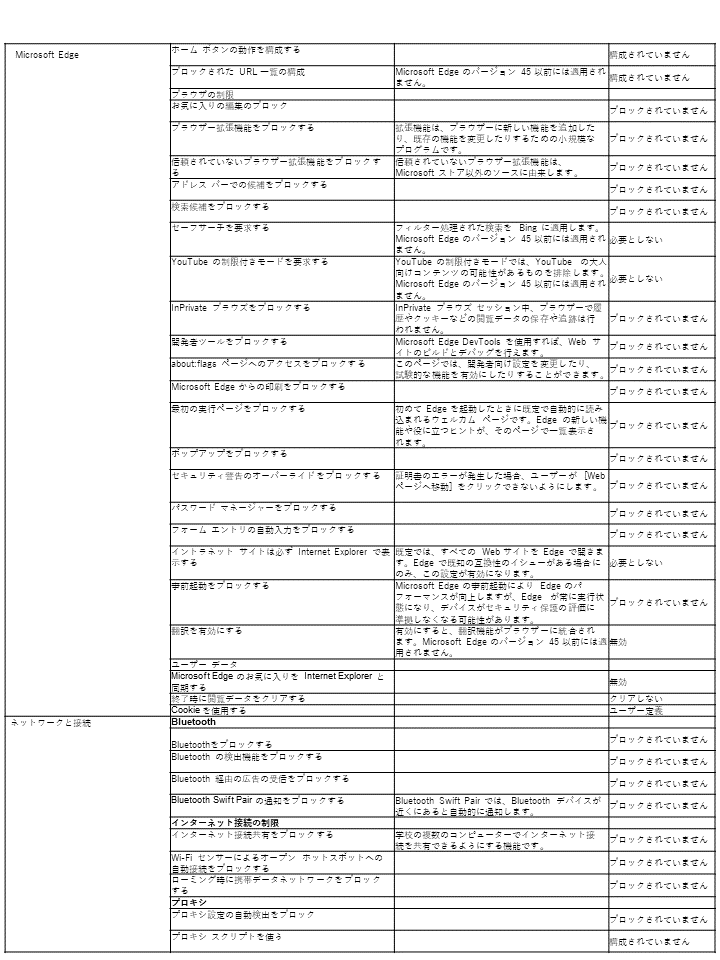
\includegraphics[width=17cm]{figures/IntuneforEducation-02.png}
\end{figure*}

\begin{figure*}[htbp]
    \centering
    \vspace{-1.5cm}
    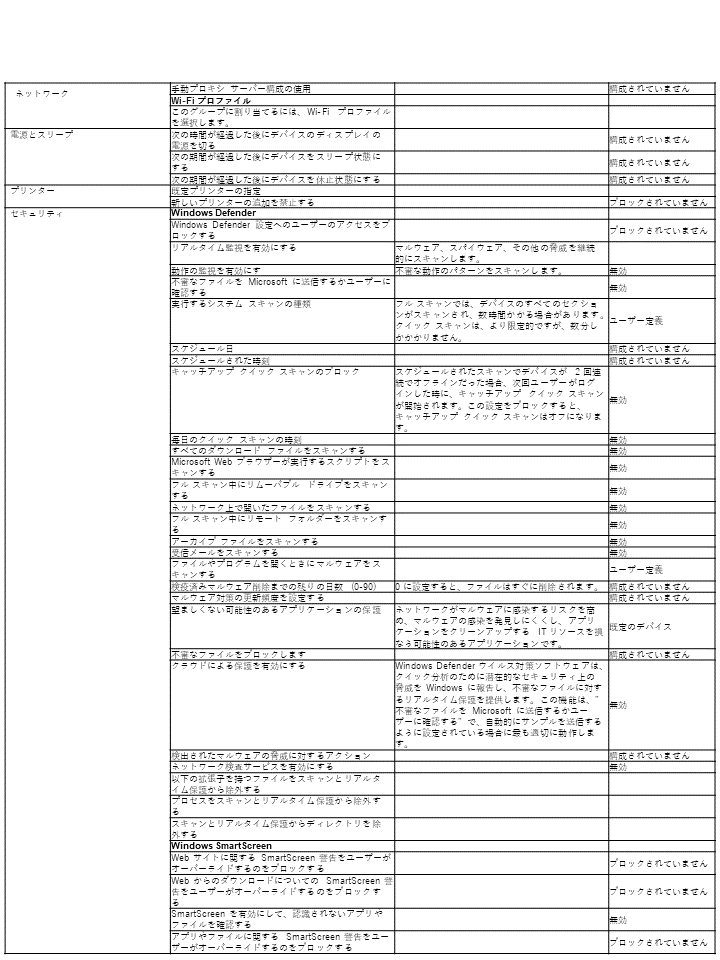
\includegraphics[width=17cm]{figures/IntuneforEducation-03.png}
\end{figure*}

\begin{figure*}[htbp]
    \centering
    \vspace{-1.0cm}
    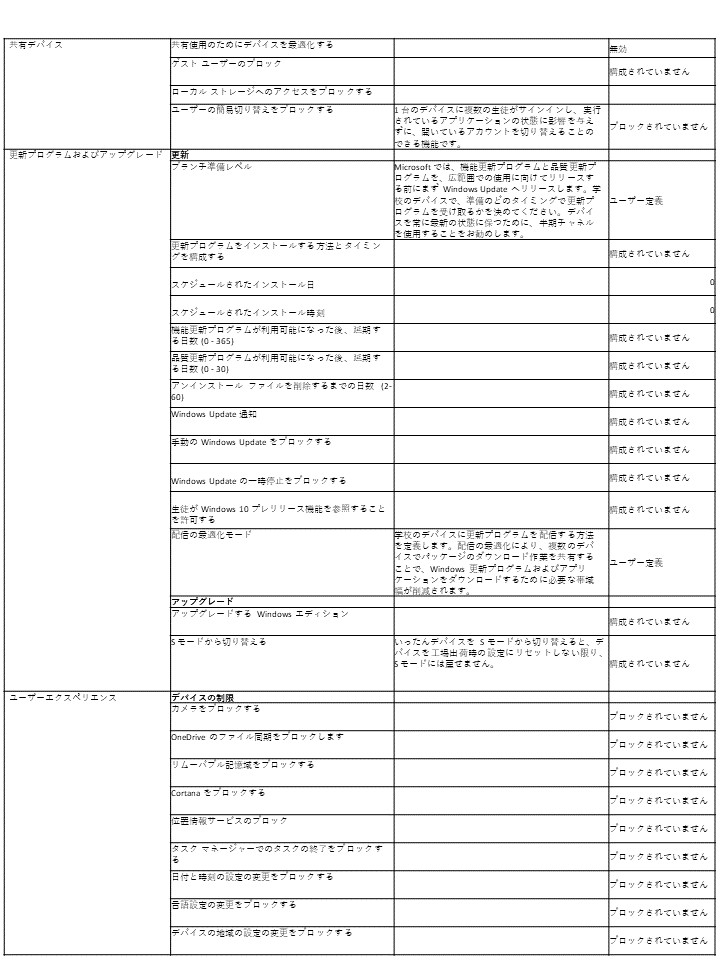
\includegraphics[width=17cm]{figures/IntuneforEducation-04.png}
\end{figure*}

\begin{figure*}[htbp]
    \centering
    \vspace{-11cm}
    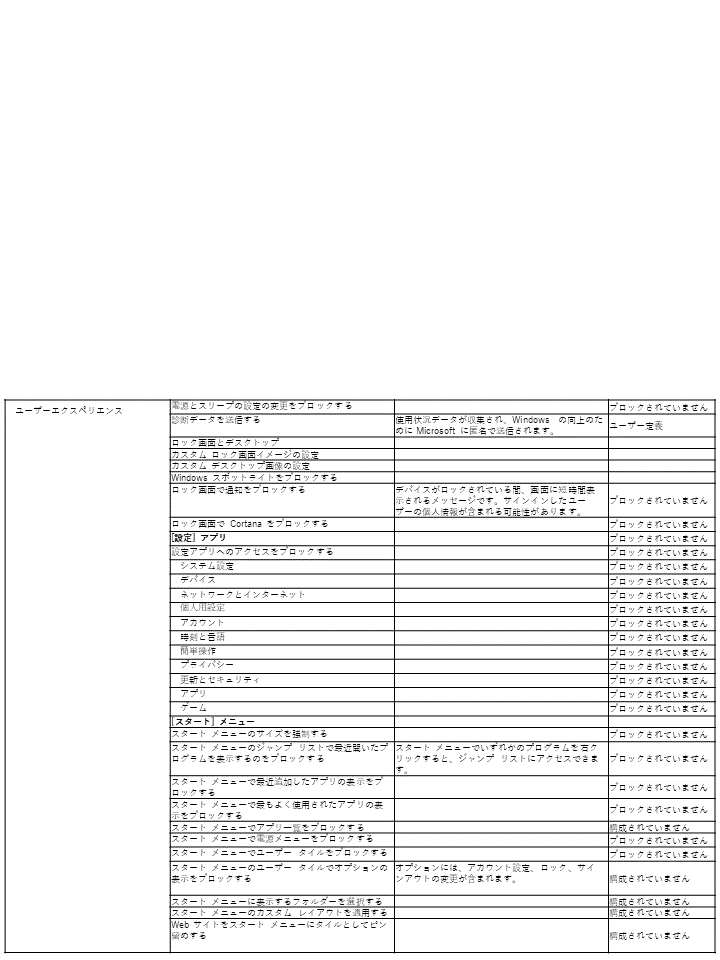
\includegraphics[width=17cm]{figures/IntuneforEducation-05.png}
    \vspace{10cm}
\end{figure*}

\begin{figure}[htbp]
    \subsection{Inturn for Education で利用できるグループ}
    
    \hspace{8pt} Intune for Education は、人、デバイス、またはそれぞれのグループに対して設定を行うことができます。例えば、先生と児童・生徒に分けてグループを作成すれば、先生と児童・生徒で異なるアプリケーションの配信したり、設定を行うことができます。グループの作成に関しては、Azure Active Directory の属性情報を基に自動的にグループにユーザーを追加する動的グループを利用することをおススメします。
\end{figure}

\begin{figure}[]
    \subsection{「高速構成」による Intune for Education の設定}

    \hspace{8pt} ここでは、\textbf{「高速構成」}を使用して、Intune for Education の設定を行いたいと思います。
\end{figure}

\begin{figure*}[h]
    \begin{minipage}{0.6\textwidth}
        \vspace{-1cm}
        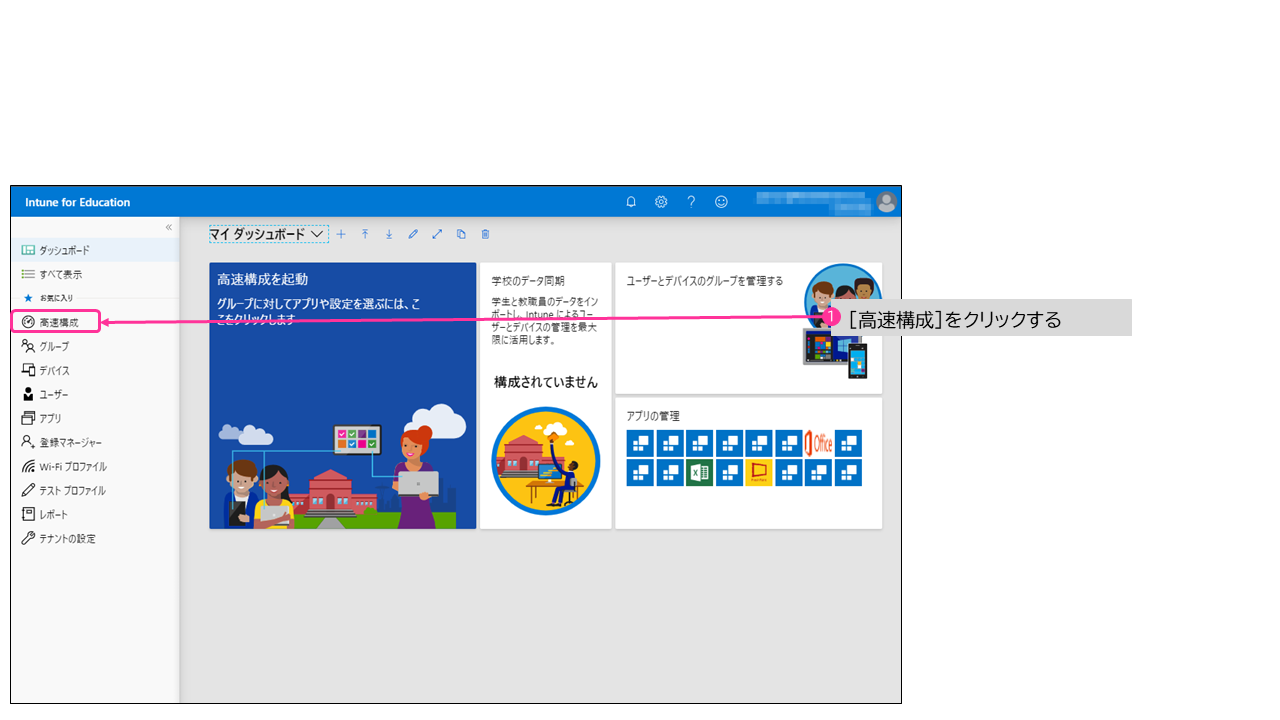
\includegraphics[width=10cm]{figures/Setup-Intune-01.png}
    \end{minipage}
    \begin{minipage}{0.4\textwidth}
        Webブラウザで \url{https://intuneeducation.portal.azure.com/}にアクセスし、Office 365 の管理者のユーザー名、パスワードでサインインしてください。\\
        サインインしたら、画面左ペインの\textbf{【高速構成】}をクリックしてください。
    \end{minipage}
\end{figure*}

\begin{figure*}[h]
    \begin{minipage}{0.6\textwidth}
        \vspace{-1cm}
        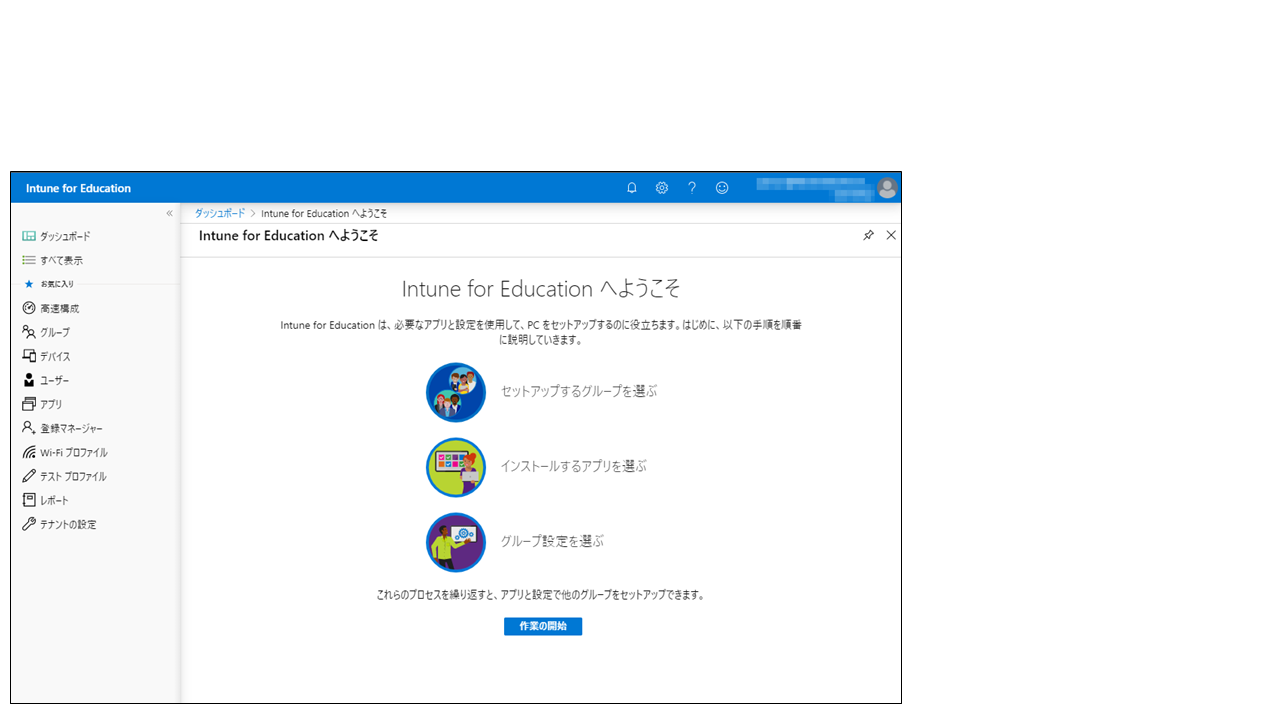
\includegraphics[width=10cm]{figures/Setup-Intune-02.png}
    \end{minipage}
    \begin{minipage}{0.4\textwidth}
        \textbf{「高速構成」}では、
        \begin{enumerate}
            \item セットアップするグループを選ぶ
            \item インストールするアプリを選ぶ
            \item グループ設定を選ぶ
        \end{enumerate}
        の3つの設定を行います。
    \end{minipage}
\end{figure*}

\begin{figure*}[h]
    \begin{minipage}{0.6\textwidth}
        \vspace{-1cm}
        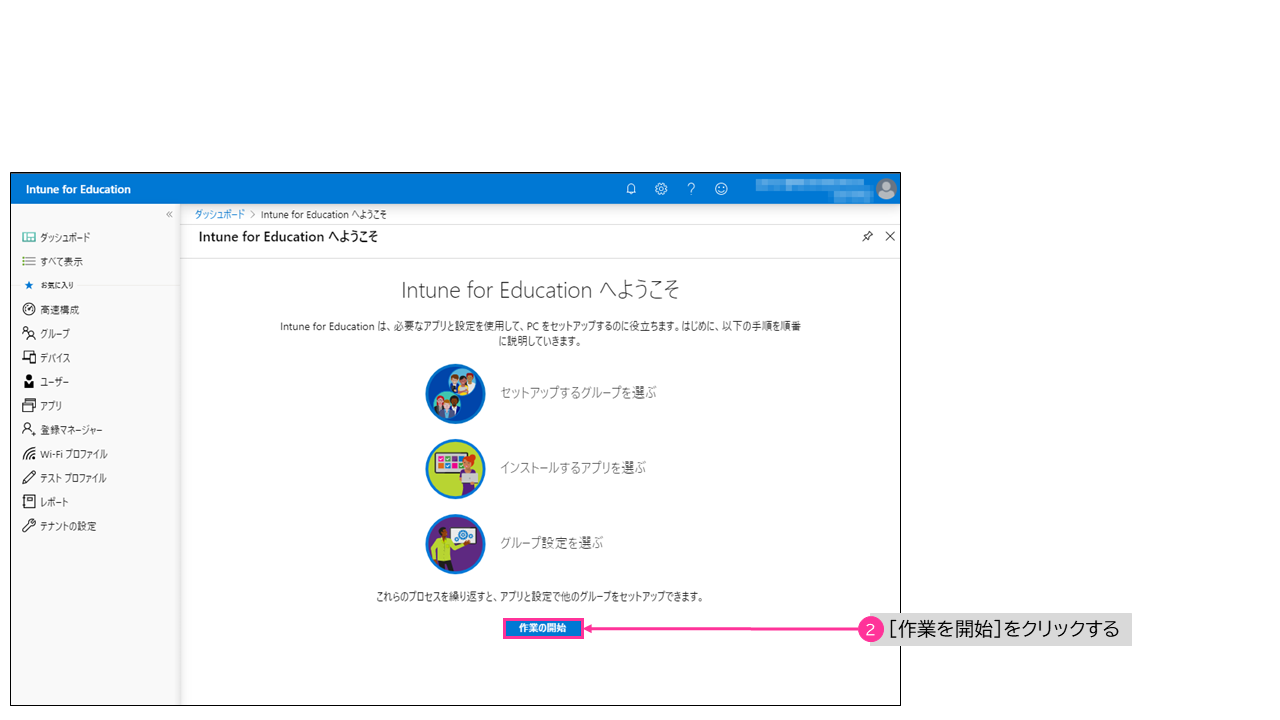
\includegraphics[width=10cm]{figures/Setup-Intune-03.png}
    \end{minipage}
    \begin{minipage}{0.4\textwidth}
        \textbf{「作業を開始」} をクリックしてください。
    \end{minipage}
\end{figure*}

\begin{figure*}[h]
    \begin{minipage}{0.6\textwidth}
        \vspace{-1cm}
        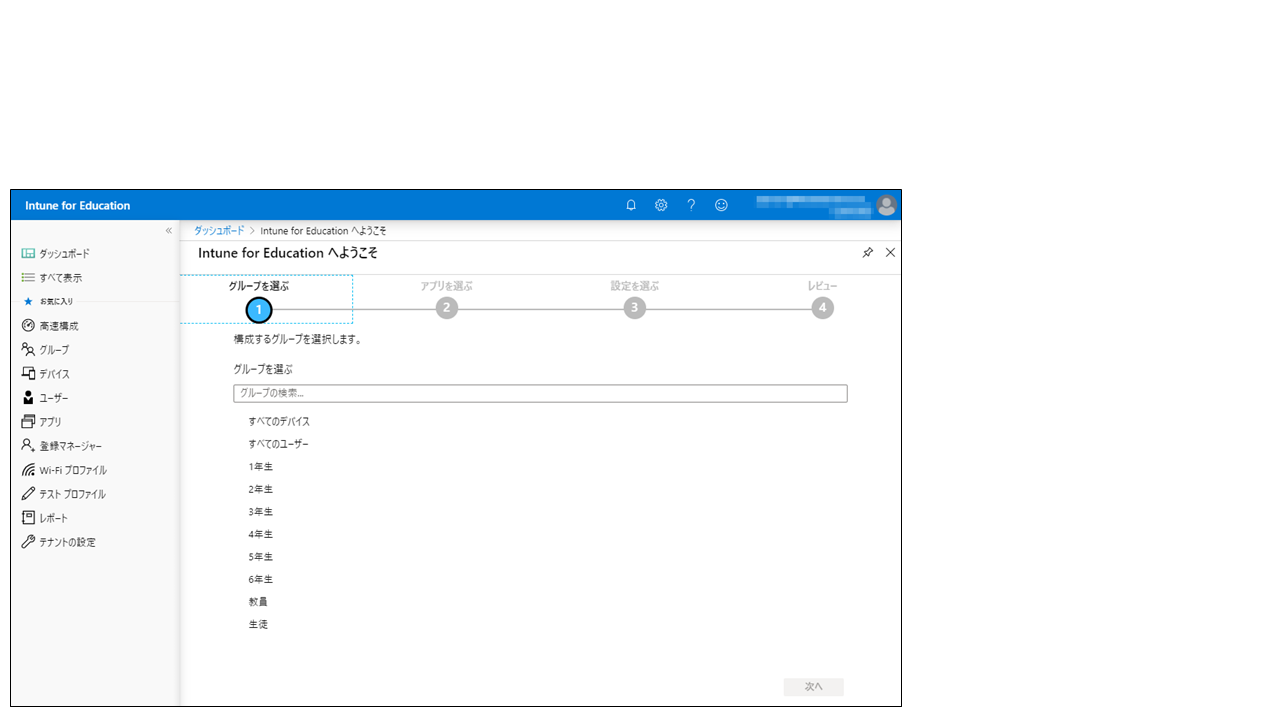
\includegraphics[width=10cm]{figures/Setup-Intune-04.png}
    \end{minipage}
    \begin{minipage}{0.4\textwidth}
        まずはじめに Intune for Education で管理するグループを選びます。グループは、Office 365のアカウント管理設定であらかじめ作成しておく必要がございます。
    \end{minipage}
\end{figure*}

\begin{figure*}[h]
    \begin{minipage}{0.6\textwidth}
        \vspace{-1cm}
        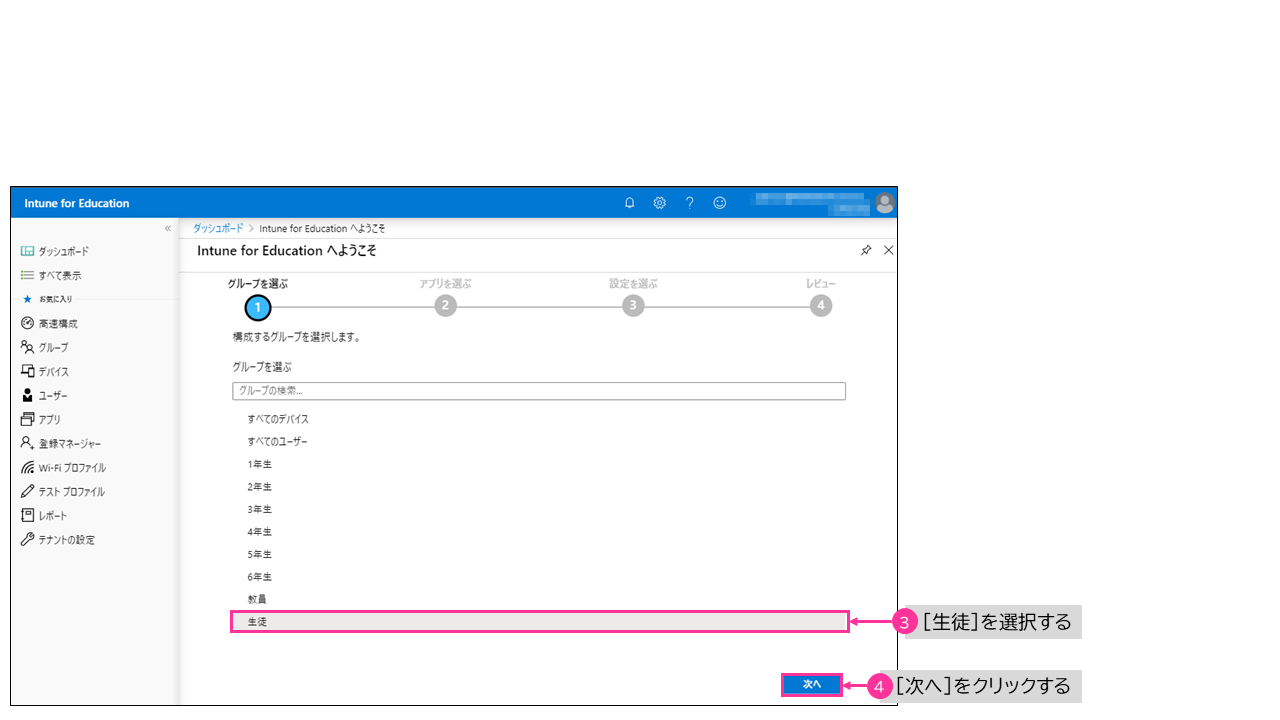
\includegraphics[width=10cm]{figures/Setup-Intune-05.png}
    \end{minipage}
    \begin{minipage}{0.4\textwidth}
        ここでは、あらかじめ生徒というグループを作成してますので「生徒」を選択し、\textbf{【次へ】}をクリックしてください。
    \end{minipage}
\end{figure*}

\begin{figure*}[h]
    \begin{minipage}{0.6\textwidth}
        \vspace{-1cm}
        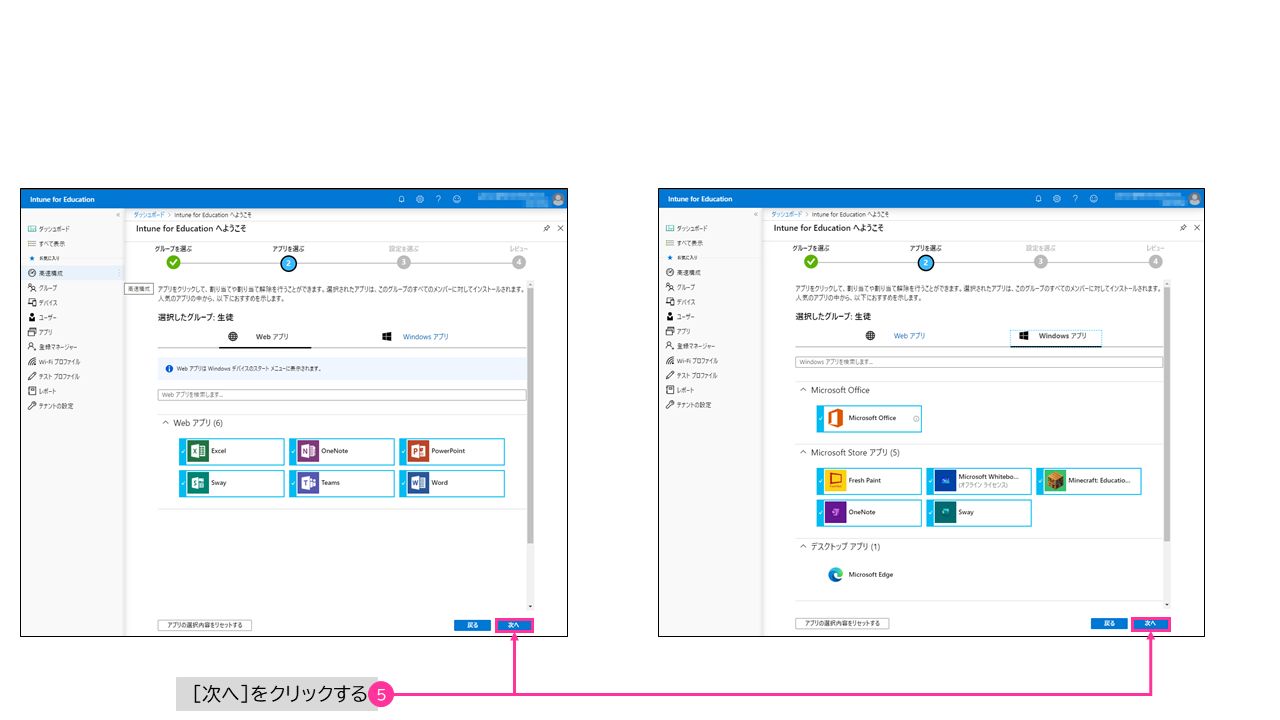
\includegraphics[width=10cm]{figures/Setup-Intune-06.png}
    \end{minipage}
    \begin{minipage}{0.4\textwidth}
        \textbf{「アプリを選ぶ」}では、Intune for Education で配布するアプリケーションを選択してください。選択が終わったら\textbf{【次へ】}をクリックしてください。
    \end{minipage}
\end{figure*}

\begin{figure*}[h]
    \begin{minipage}{0.6\textwidth}
        \vspace{-1cm}
        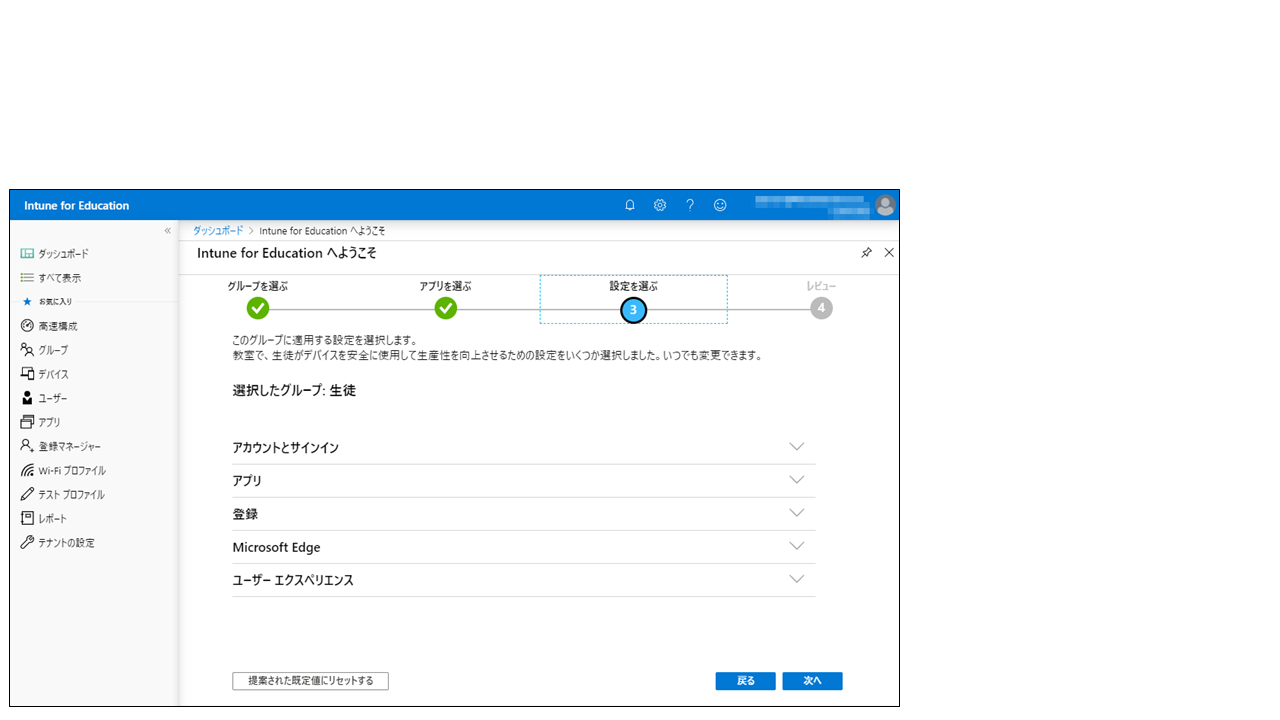
\includegraphics[width=10cm]{figures/Setup-Intune-07.png}
    \end{minipage}
    \begin{minipage}{0.4\textwidth}
        \textbf{「設定を選ぶ」}では、
        \begin{enumerate}
            \item アカウントとサインイン
            \item アプリ
            \item 登録
            \item Microsoft Edge
            \item ユーザーエクスペリエンス
        \end{enumerate}
        の5つの設定を行います。
    \end{minipage}
\end{figure*}

\begin{figure*}[h]
    \begin{minipage}{0.6\textwidth}
        \vspace{-1cm}
        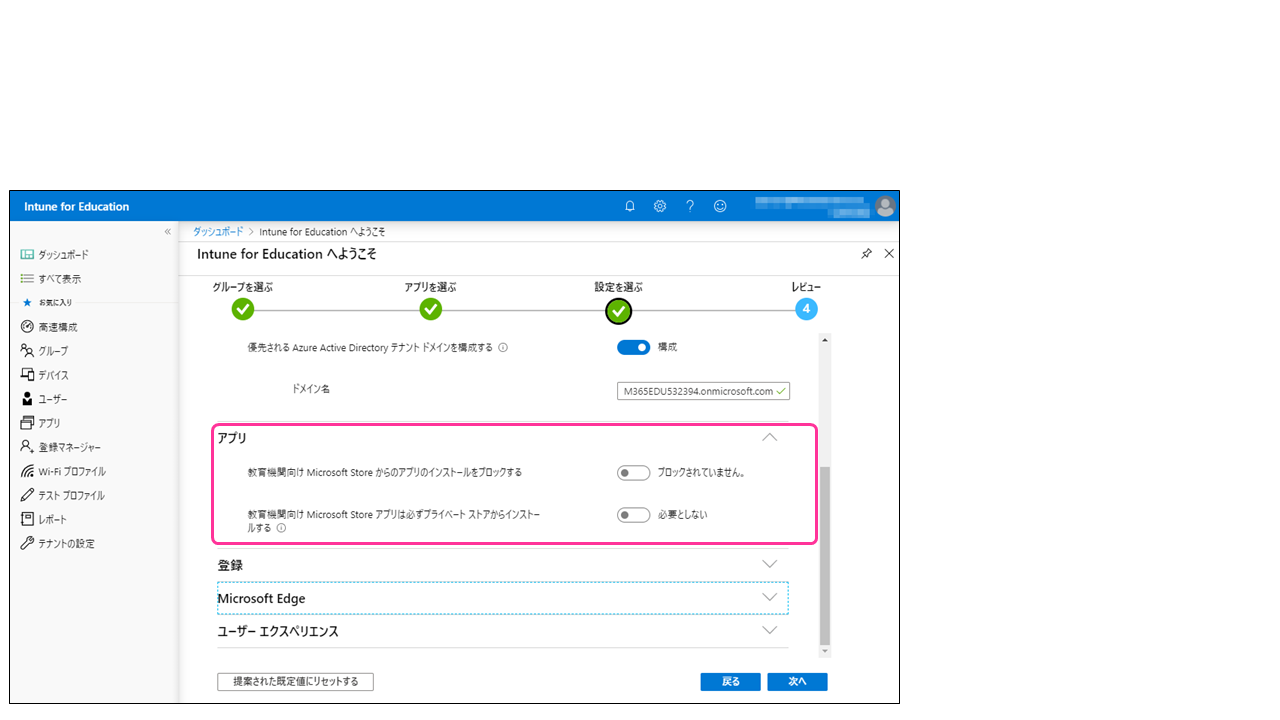
\includegraphics[width=10cm]{figures/Setup-Intune-09.png}
    \end{minipage}
    \begin{minipage}{0.4\textwidth}
       \textbf{「アプリ」}では、
       \begin{enumerate}
           \item 教育機関向け Microsoft Store からのアプリのインストールをブロックする
           \item 教育機関向け Microsoft Store アプリは必ずプライベート ストアからインストールする
       \end{enumerate}
       この2つのポリシーを設定することができます。
    \end{minipage}
\end{figure*}

\begin{figure*}[h]
    \begin{minipage}{0.6\textwidth}
        \vspace{-1cm}
        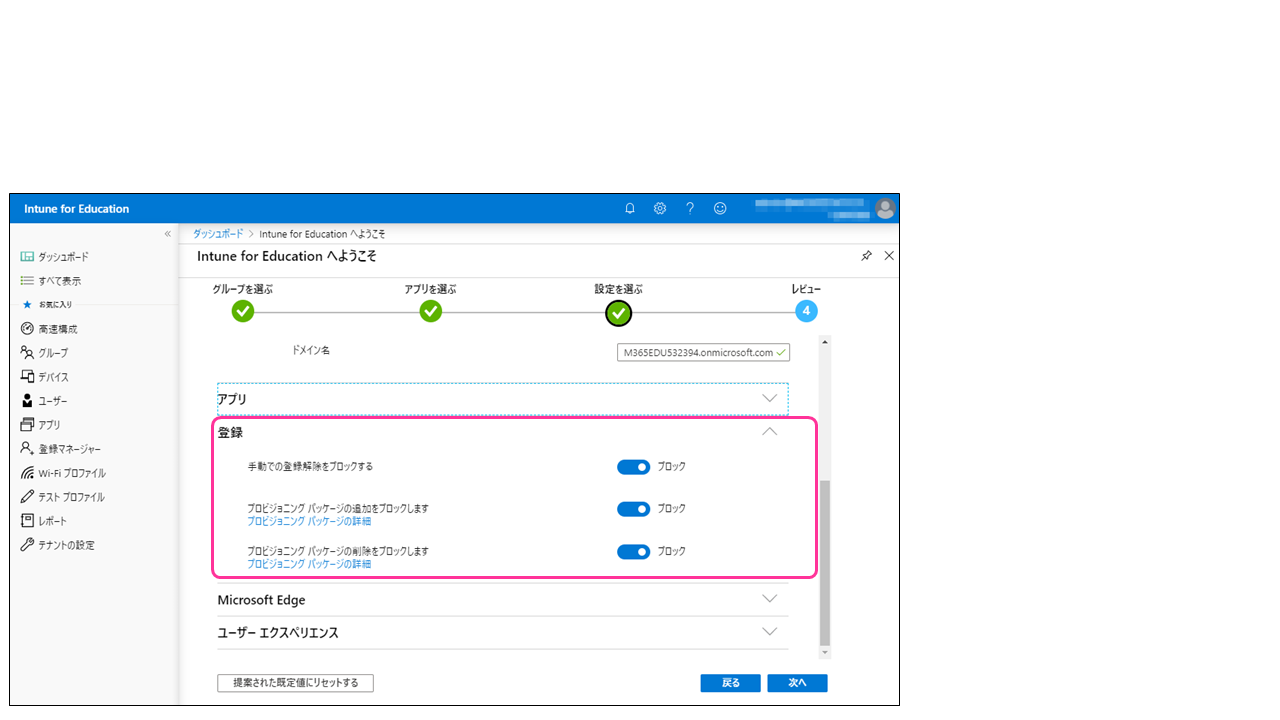
\includegraphics[width=10cm]{figures/Setup-Intune-10.png}
    \end{minipage}
    \begin{minipage}{0.4\textwidth}
        \textbf{「登録」}では、デバイスを Azure Active Directory に登録するためのポリシーを設定することができます。
    \end{minipage}
\end{figure*}

\begin{figure*}[h]
    \begin{minipage}{0.6\textwidth}
        \vspace{-1cm}
        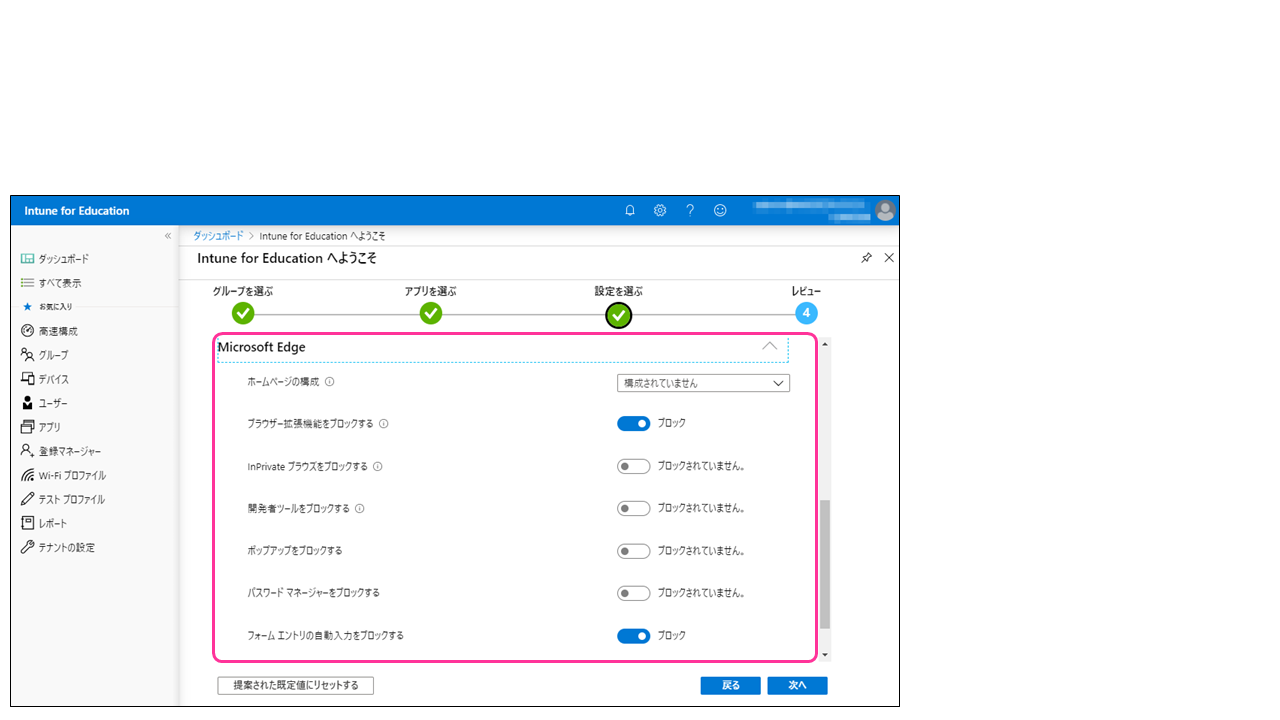
\includegraphics[width=10cm]{figures/Setup-Intune-11.png}
    \end{minipage}
    \begin{minipage}{0.4\textwidth}
       \textbf{「Microsoft Edge」}では、Microsoft Edge に関連する様々なポリシーを設定することができます。
    \end{minipage}
\end{figure*}

\begin{figure*}[h]
    \begin{minipage}{0.6\textwidth}
        \vspace{-1cm}
        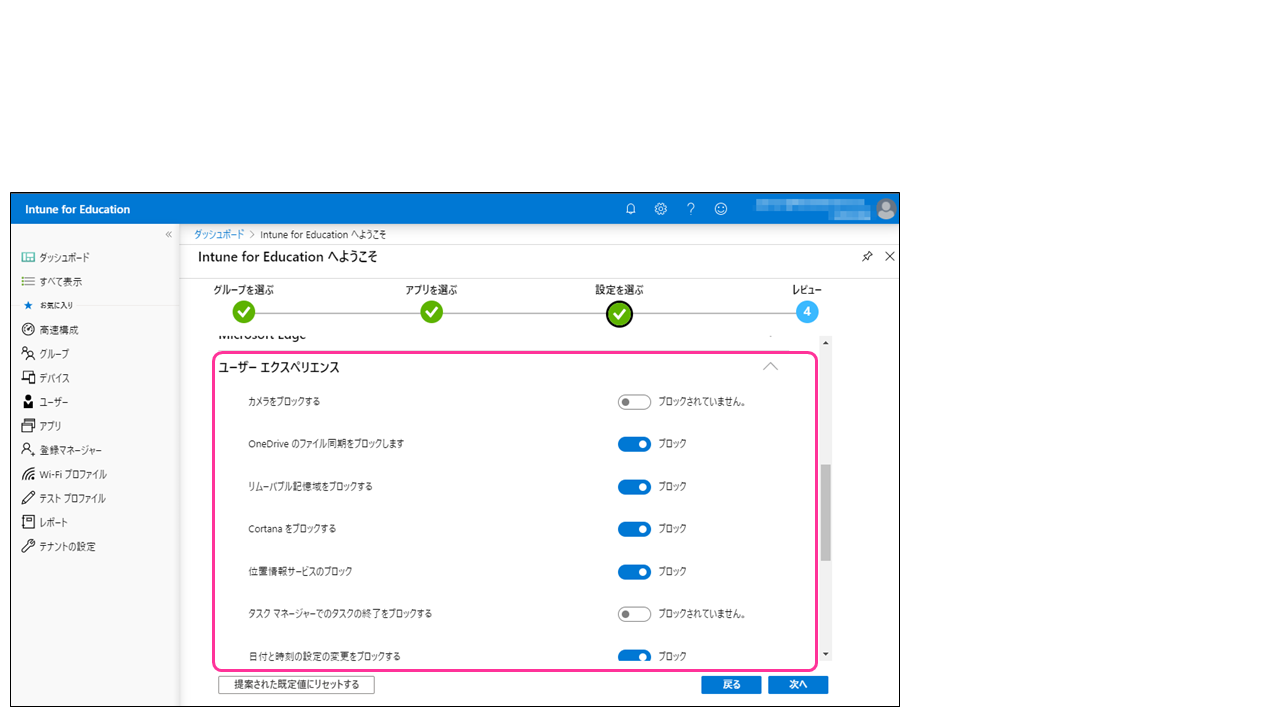
\includegraphics[width=10cm]{figures/Setup-Intune-12.png}
    \end{minipage}
    \begin{minipage}{0.4\textwidth}
       \textbf{「ユーザーエクスペリエン」}では、ユーザーエクスペリエンに関する様々なポリシーを設定することができます。
    \end{minipage}
\end{figure*}

\begin{figure*}[h]
    \begin{minipage}{0.6\textwidth}
        \vspace{-1cm}
        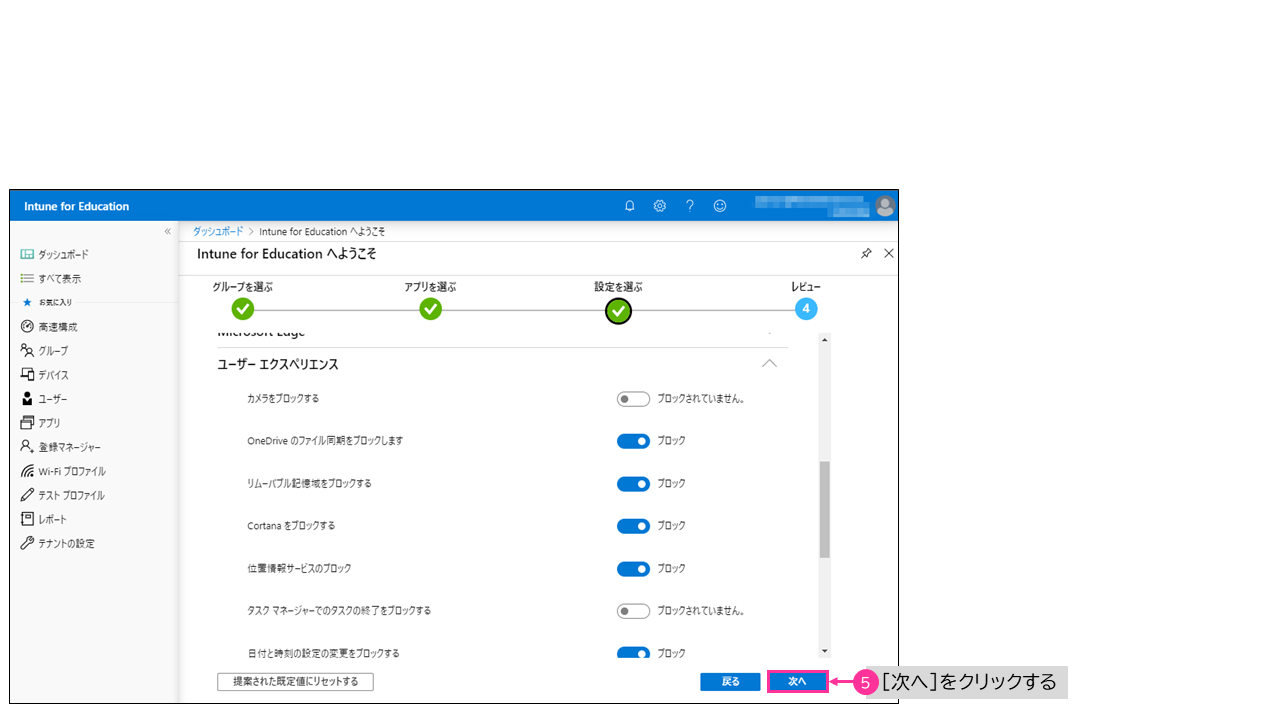
\includegraphics[width=10cm]{figures/Setup-Intune-13.png}
    \end{minipage}
    \begin{minipage}{0.4\textwidth}
        すべての設定が完了したら\textbf{【次へ】}をクリックしてください。
    \end{minipage}
\end{figure*}

\begin{figure*}[h]
    \begin{minipage}{0.6\textwidth}
        \vspace{-1cm}
        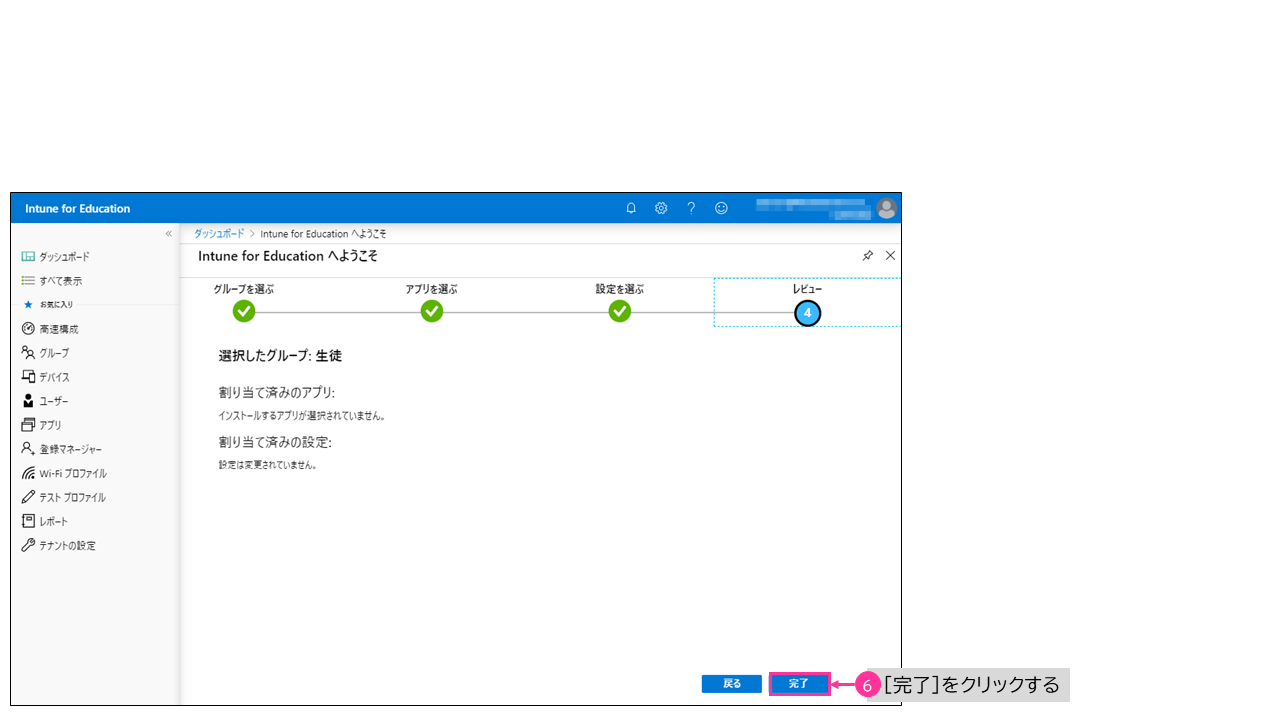
\includegraphics[width=10cm]{figures/Setup-Intune-14.png}
    \end{minipage}
    \begin{minipage}{0.4\textwidth}
        最後に\textbf{【完了】}をクリックしてください。
    \end{minipage}
\end{figure*}

\begin{figure*}[h]
    \begin{minipage}{0.6\textwidth}
        \vspace{-1.5cm}
        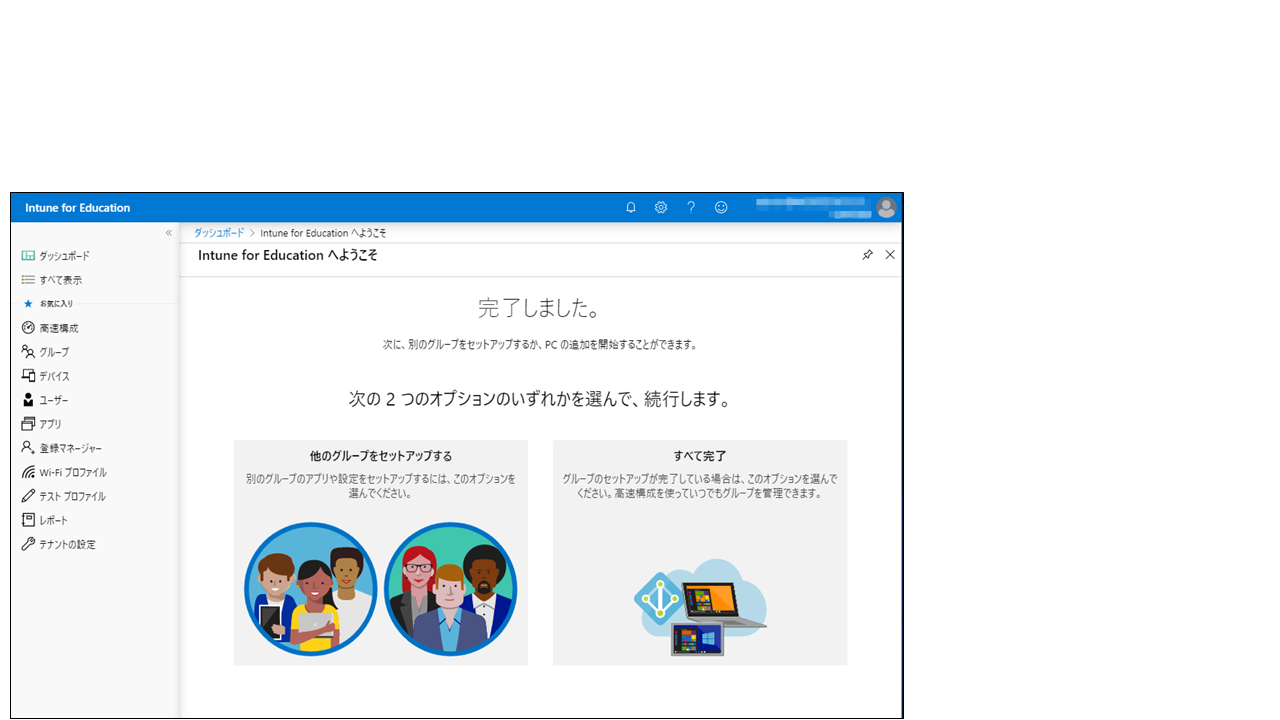
\includegraphics[width=10cm]{figures/Setup-Intune-15.png}
    \end{minipage}
    \begin{minipage}{0.4\textwidth}
        他のグループのポリシーを設定したい場合には、他のグループをセットアップするクリックしてしてください。そうでない場合には、「すべて完了」をクリックしてください。\\
        これで高速構成の設定は完了しました。あとは生徒が端末にはじめてログインしたときに、これらの設定が端末に適用されます。
    \end{minipage}
\end{figure*}